\section{Introduction}
\label{introduction}

High pressure flexible hoses, reinforced by braided metallic or fabric wires, are utilized in a variety of engineering applications, to transmit fluid in aircrafts, automobiles and typical hydraulic systems. 
These hoses are practically employed in more severe conditions, where high pressure loads, commonly of the order of tens of MPa,  are not static but periodically or randomly fluctuating, and furthermore thermal loading, vibration and large deformation are coupled with the pressure[]. 



The construction of such a hose is illustrated in Fig.\ref{fig:Hose-Structure}. It comprises an inner tube core, mostly PTFE, covered with layers of high tensile steel wires wounding around it, such that the PTFE resists leakage and chemical corrosion while the steel wires layers act as the principle load-carrying elements. These reinforcement layers can be classified into helix-wounds and braids. 






Braided structures can be categorized as diamond ($ 1 \times 1 $ repeat), regular ($ 2 \times 2 $ repeat) and hercules ($ 3 \times 3 $ repeat) based on the weave pattern \cite{Rawal:2015dq}  and the regular braids are most widely produced for high pressure flexible hose on circular braiding machines.
Regular braids  are also known as biaxial braids, consisting of two sets of braider strands, which are aligned in the bias angle to the axis, namely the braid angle, which play a pivot part in defining the performance of the hose under pressure.[1]

\begin{figure}[h]
\centering
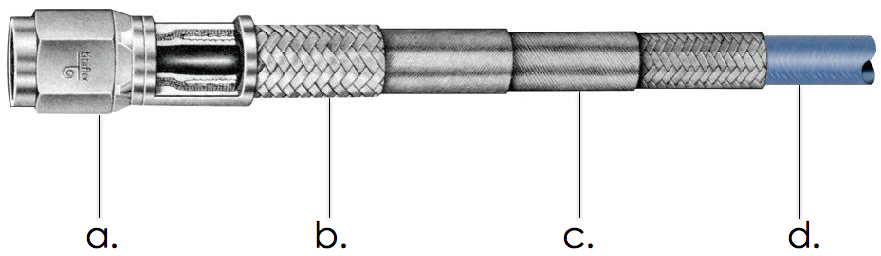
\includegraphics[width=0.7\linewidth]{figures/Hose-Structure}
\caption{Hose Structure}
\label{fig:Hose-Structure}
\end{figure}





The helix-wound layers are wounded in pairs, one layer of each pair being wound left hand and the other right hand in order to achieve a torque balanced construction (i.e. minimal twist on pressurization)[]. There are no intermediate layers of plastic and wires in the same layer are touching in order for maximum packing density.



In conventional braider, spindle carriers rotate along a circular track. Half of the carriers travel in clockwise direction, with the others in the reverse direction, similar to maypole arrangement (see Figure 1).As a result, he two sets of spindles interlace with each other at a bias angle to the tube axis, namely the braid angle, which play a pivot part in defining the performance of the hose under pressure.[1]
The tube in Figure 1 is designed a hybrid structure with both the helix-wound reinforcement and the braid reinforcement, to have sufficient structural safety against extremely high pressure. They may be independently used in middle-high pressure hose. Braided fiber yarns, especially Kevlar [], has been used instead of metallic wires, for its light weight. Effects have been made to model and characterize the mechanical and structural elements of the three reinforcement methods respectively.



